\chapter{Measurement Methodology}

This chapter is dedicated to answering the questions of what was measured and how results were obtained. Firstly, the measurement setup is discussed in view of the necessity to verify the recorded data. Subsequently,  the GNU Radio flowgraphs are explained. Secondly, with reference to the flowgraphs measurement metrics are formally defined.  Lastly, an overview of the semi-automatic measurement script system designed to automate, therefore accelerate the process of file system management, data processing and result plotting is given.

\section{Measurement Setup}

The setup consists of two USRP2s from Ettus Research and two USRP 2920s from National Instruments. Where the former pair is programmed as receiver and sniffer and the latter  as senders as depicted in \ref{fig:measurement-setup}. Each USRP was connected to a gigabit switch through a LAN cabel. The scripts running on the devices were launched from the institute's computer with the IP 134.130.223.151, which was remote controlled from my private laptop. Table \ref{tab:measurement-parameters} contains other necessary information to reproduce the measurement results.

\begin{figure}[tb]
	\label{fig:measurement-setup}
	\begin{center}
		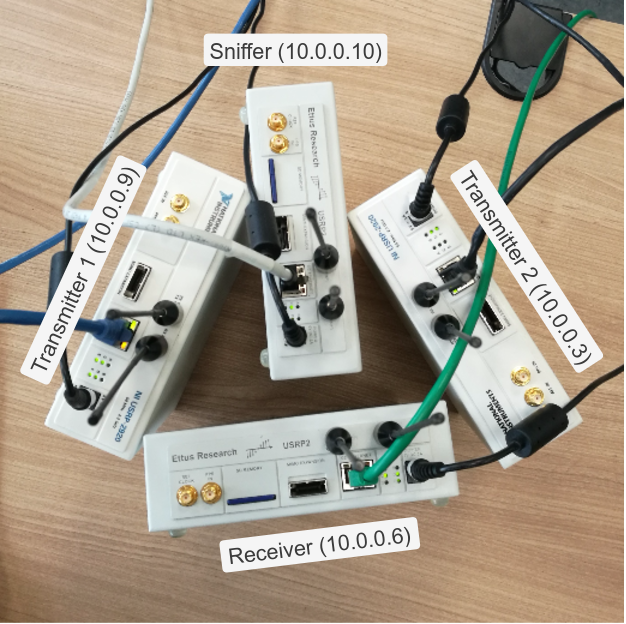
\includegraphics[width=0.5\textwidth]{pictures/measurement_setup}
	\end{center}
	\caption{Photo of the measurement setup}
\end{figure}

% Measurement parameters
\begin{table}
	\label{tab:measurement-parameters}
	\begin{center}
		\begin{tabular}{p{2.5cm}p{2cm}p{2cm}p{1.5cm}p{1.5cm}p{2cm}}
			\toprule
			Function & TX Gain & RX Gain & Source Address & Dest. Address & IP Address\\
			\midrule
			Receiver 		& 4dB 	& 10dB 	& X 	& any	& 10.0.0.6\\
			Sniffer 		& 0 	& 0 	& any 	& any	& 10.0.0.10 \\
			Transmitter 1 	& 5dB 	& 0 	& Y 	& 	X 	& 10.0.0.9 \\
			Transmitter 2	& 9dB 	& 0 	& Z 	& 	X 	& 10.0.0.3 \\
			\bottomrule	
		\end{tabular}\caption{Setup parameters}
	\end{center}
\end{table}


\section{GNU Radio Flowgraphs}

%\subsection{Common Variables}
%
%Our GNU Radio pure ALOHA and non-persistent/1-persistent CSMA implementations are placed on top of a common PHY layer warranting comparability. The specific PHY layer implementation is beyond this work's scope, but a few parameters common to all flowgraphs shall be discussed nonetheless. Hereinafter, these variables and their values will not be mentioned unless they are important concerning the interpretation of results.
%
%\begin{figure}[ht]
%	\label{fig:grc-common-variables}
%	\begin{center}
%		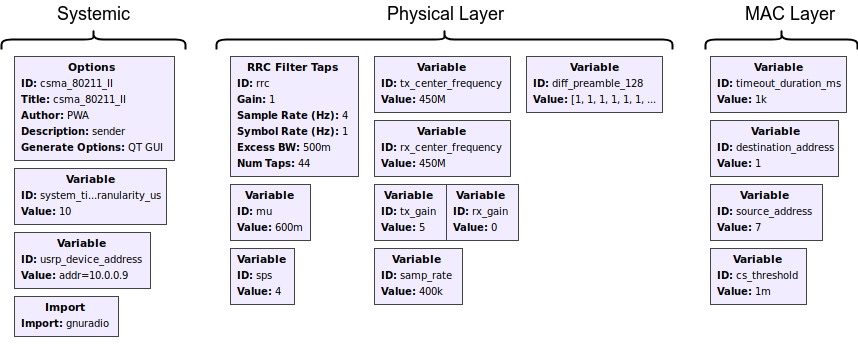
\includegraphics[width=\textwidth]{pictures/grc_common_variables}
%	\end{center}
%\caption{Variables Common to All Flowgraphs}
%\end{figure}     

\subsection{Receiver and Sniffer}

Figure \ref{fig:grc-receiver} shows the two-way handshake receiving logic. After frame integrity is checked and type is confirmed to be data frame an acknowledgment is generated. The \texttt{frame\_probe} blocks record the times when the frames reach certain positions in the flowgraph representing the occurrence of events such as frame reception, passed or failed frame integrity check and more. Note that the address check is disabled so that the receiver may receive frames from any sender.

The sniffer consists only of a single \texttt{frame\_probe} block, which records detected power above noise level during the whole measurement. The sniffer provides valuable insight of what is actually going on in the channel from a "neutral" point of view. Neutral in the sense of:

\begin{itemize}
	\item A clear distinction between the senders can be made according to the energy levels, since the sniffer is located between the senders and transmission gains were chosen accordingly.
	\item Sensing the channel is possible during the whole measurement time, because the sniffer is never sending.
\end{itemize}

In a nutshell, the sniffer is a valuable debugging and verification tool as described in more detail in section \ref{sec:measurement-metrics}.

\begin{sidewaysfigure}[ht]
	\label{fig:grc-receiver}
	\begin{center}
		\subfloat[Receiver]{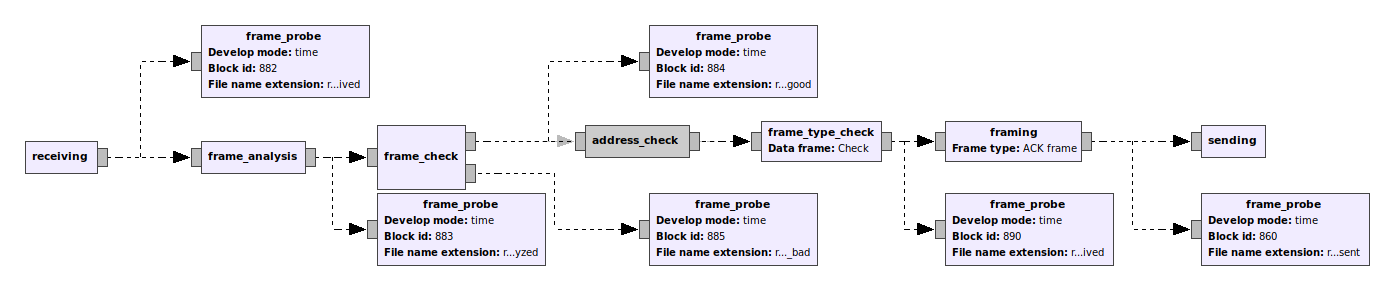
\includegraphics[width=\textwidth]{pictures/grc_receiver_flowgraph}}
		\vskip 40pt
		\subfloat[Sniffer]{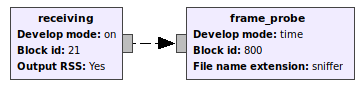
\includegraphics[width=0.3\textwidth]{pictures/grc_sniffer_flowgraph}}
	\end{center}
	\caption{GRC Receiver Flowgraphs}
\end{sidewaysfigure}

\subsection{Pure ALOHA Transmitter}
The \texttt{run} block enables us to start several senders exactly at the same time, which is useful if we execute the flowgraphs manually without the automated measurement scripts. Payload is generated in the \texttt{dummy\_source} block, packed into a frame in the \texttt{framing} block and buffered in the \texttt{frame\_buffer} block. The interval between generated frames is determined by a \texttt{general\_timer} block, which we trigger either constant or exponentially distributed intervals. Self-reception is prevented by shutting down the receiver when about to send a frame through the sending block. As soon as the data packet is sent off the \texttt{timeout} block receives a copy of the data frame. If the timeout timer is reset by a recevied ACK before it runs out the next frame in the buffer is dequeued, otherwise the data is forwarded to the \texttt{resend\_check} block. If the maximum number of retransmissions, in our case 6 has not been reached a retransmission is issued, otherwise the frame is dropped without substitution.

\begin{sidewaysfigure}[h]
	\label{fig:grc-aloha-sender}
	\begin{center}
		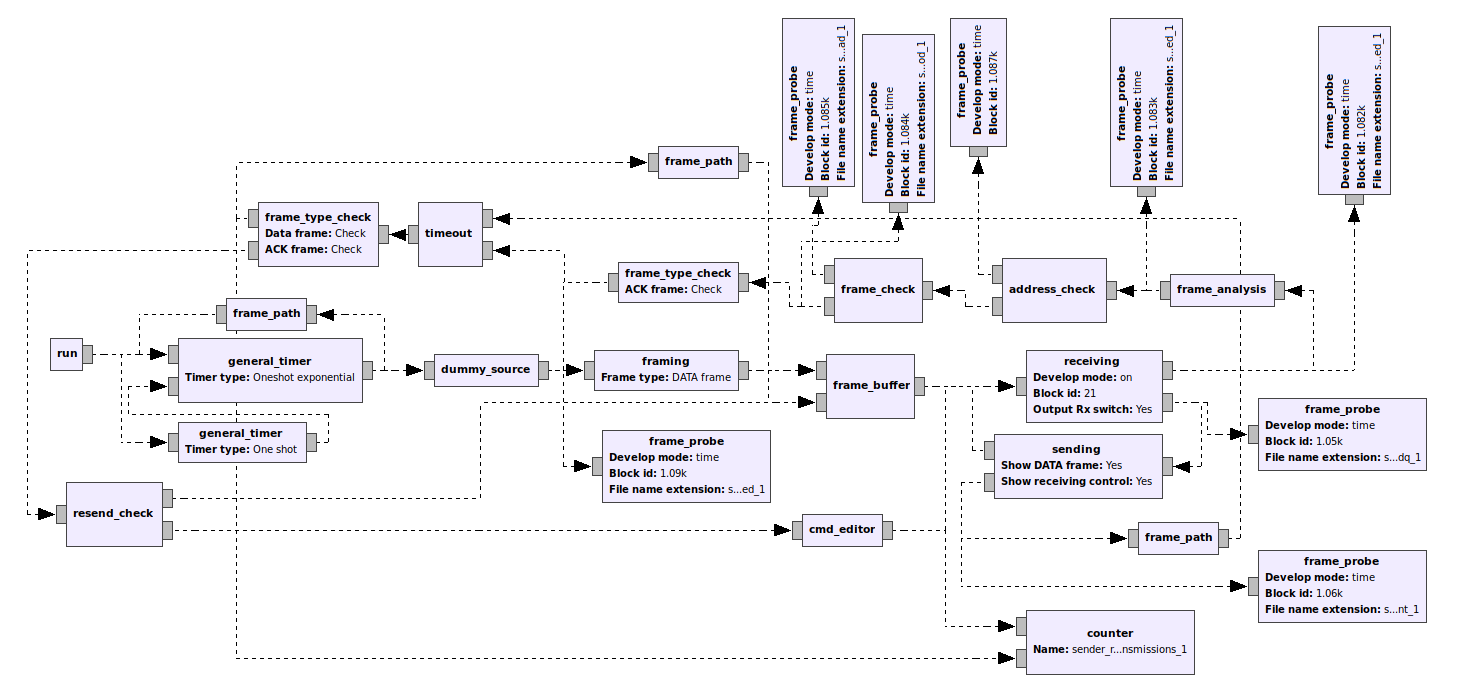
\includegraphics[width=\textwidth]{pictures/grc_aloha_transmitter_flowgraph}
\end{center}
\caption{GRC Pure ALOHA Transmitter Flowgraph}
\end{sidewaysfigure}

\subsection{CSMA Transmitter}

The CSMA flowgraph aims at resembling 802.11 DCF and features CCA through thresholding in the \texttt{carrier\_sensing} block. Despite the fact that this block has the feature of adaptively determining an appropriate carrier sensing threshold we chose a fixed value of 0.002 power units (PU) \footnote{Power unit is a linear-scale unit read out via the UHD driver.}. This choice was made to make sure that ALOHA transmission power levels were not confused with noise during the adaptive CSMA noise floor detection period. 

DIFS and SIFS are realized through \texttt{general\_timer} blocks with the respective values. The design, as depicted, does not feature the RTS/CTS exhange.

\begin{sidewaysfigure}[h]
	\label{fig:grc-csma-sender}
	\begin{center}
		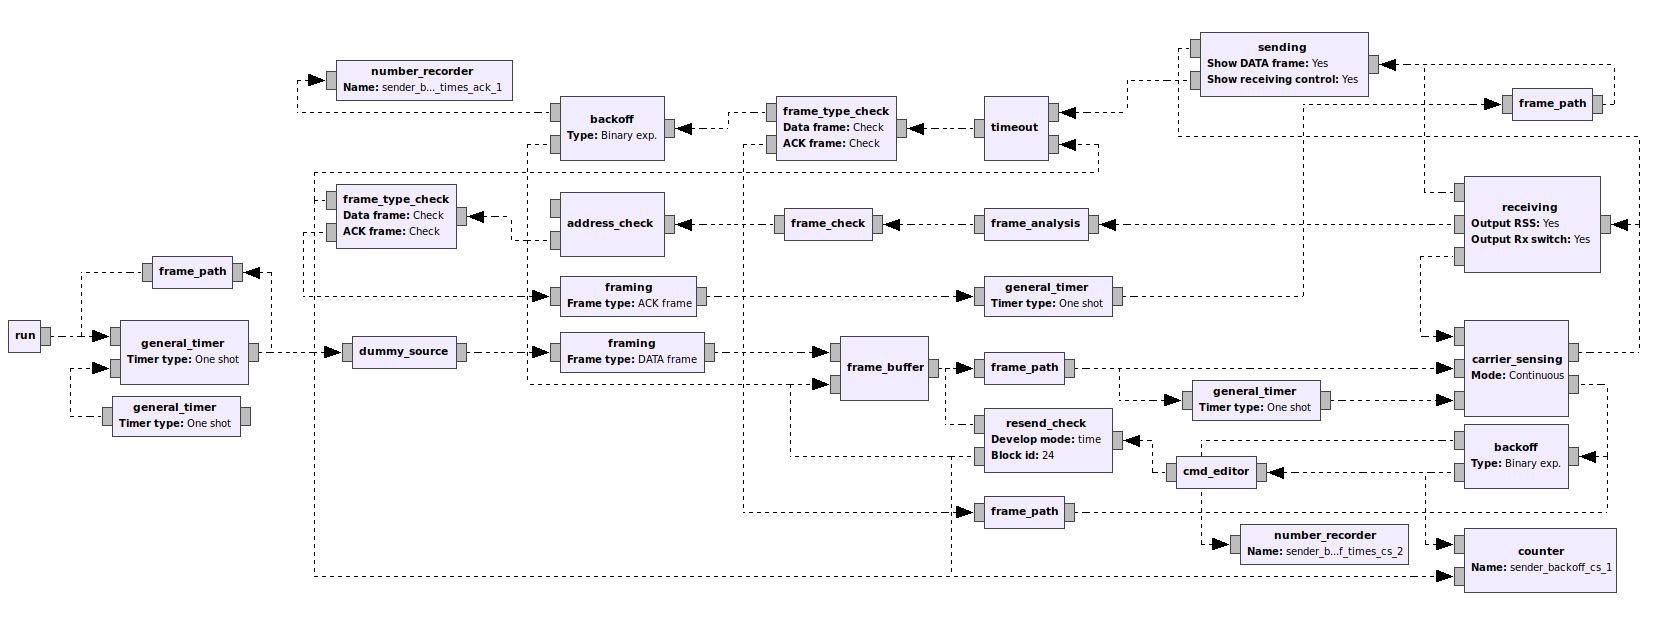
\includegraphics[width=\textwidth]{pictures/grc_csma_transmitter_flowgraph}
\end{center}
\caption{GRC CSMA Transmitter Flowgraph}
\end{sidewaysfigure}

\clearpage

\section{Measurement Metrics}
\label{sec:measurement-metrics}

All recorded metrics will be defined in this section. Furthermore, we will describe the way how they were obtained and how we verified them.

\subsection{Throughput}

\subsection{Round-Trip Time}

\subsection{Backoff Times}

\subsection{Channel Energy Level}

\subsection{Packet Durations}

\section{Measurement Script System}
\label{sec:script-system}

\begin{figure}[ht]
	\label{fig:script-system}
	\begin{center}
		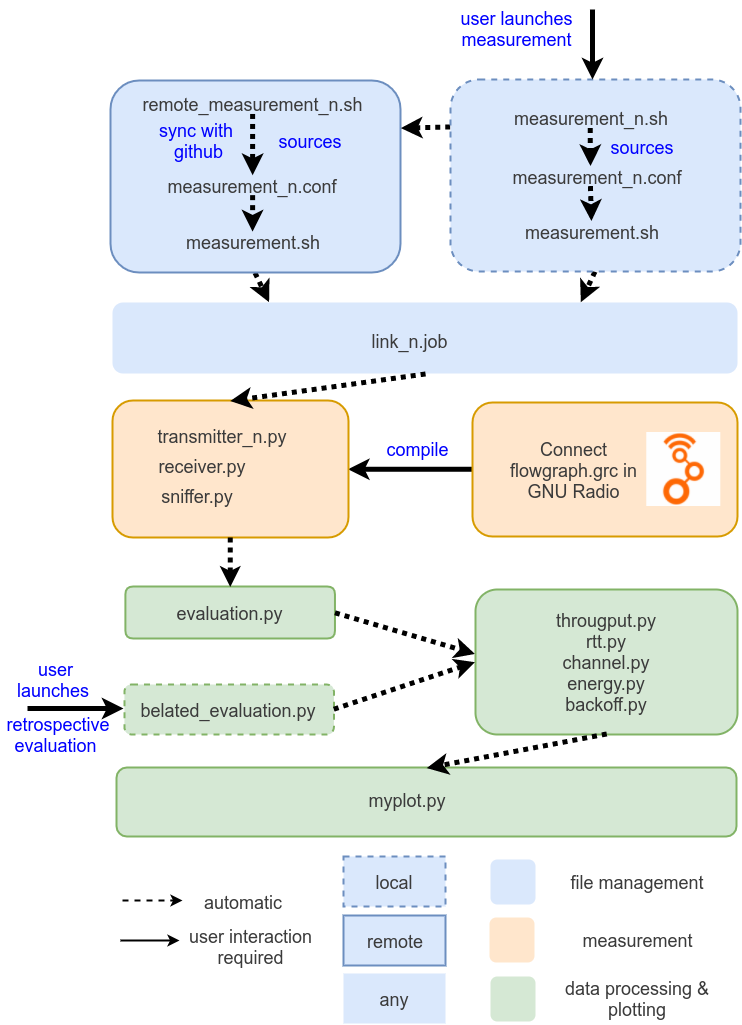
\includegraphics[width=0.65\textwidth]{pictures/script_system}
	\end{center}
	\caption{The three-phase measurement script system}
\end{figure}